\subsection{Dataset}

We choose data from Stanford Large Network Dataset Collection, including social network, collaboration network and peer-to-peer network data.

\begin{table}[H]
	\begin{tabular}{| l | l | l | l | p{7cm} |}
	  \hline			
	  dataset & Type & Nodes & Edges & Description \\ \hline
	  ego-Facebook & Undirected & 4,039 & 88,234 & Social circles from Facebook (anonymized) \\ \hline
	  wiki-Vote & Directed & 7,115 & 103,689 & Wikipedia who-votes-on-whom networt \\ \hline
	  ca-GrQc & Undirected & 5,242 & 14,496 & Collaboration network of Arxiv General Relativity \\ \hline
	  ca-HepTh & Undirected & 9,877	& 25,998 & Collaboration network of Arxiv High Energy Physics Theory \\ \hline
	  p2p-Gnutella08 & Directed & 6,301 & 20,777 & Gnutella peer to peer network from August 8 2002 \\
	  \hline  
	\end{tabular}
\end{table}


\subsection{Performance}

In the following sections, we present the performance of different indexing methods \{non-clustering index on \texttt{source}, clustering index on \texttt{source}, composite index on \texttt{source} and \texttt{destination}\} $\times$ different node ordering methods \{random ordering, coreness ordering, pagerank ordering\}.

\subsubsection{Undirected Social Network: Facebook}

Facebook dataset has more edges and a long tail in degree distribution, hence it takes relatively longer run-time for our algorithms compared with other networks.

\begin{figure}[H]
\centering
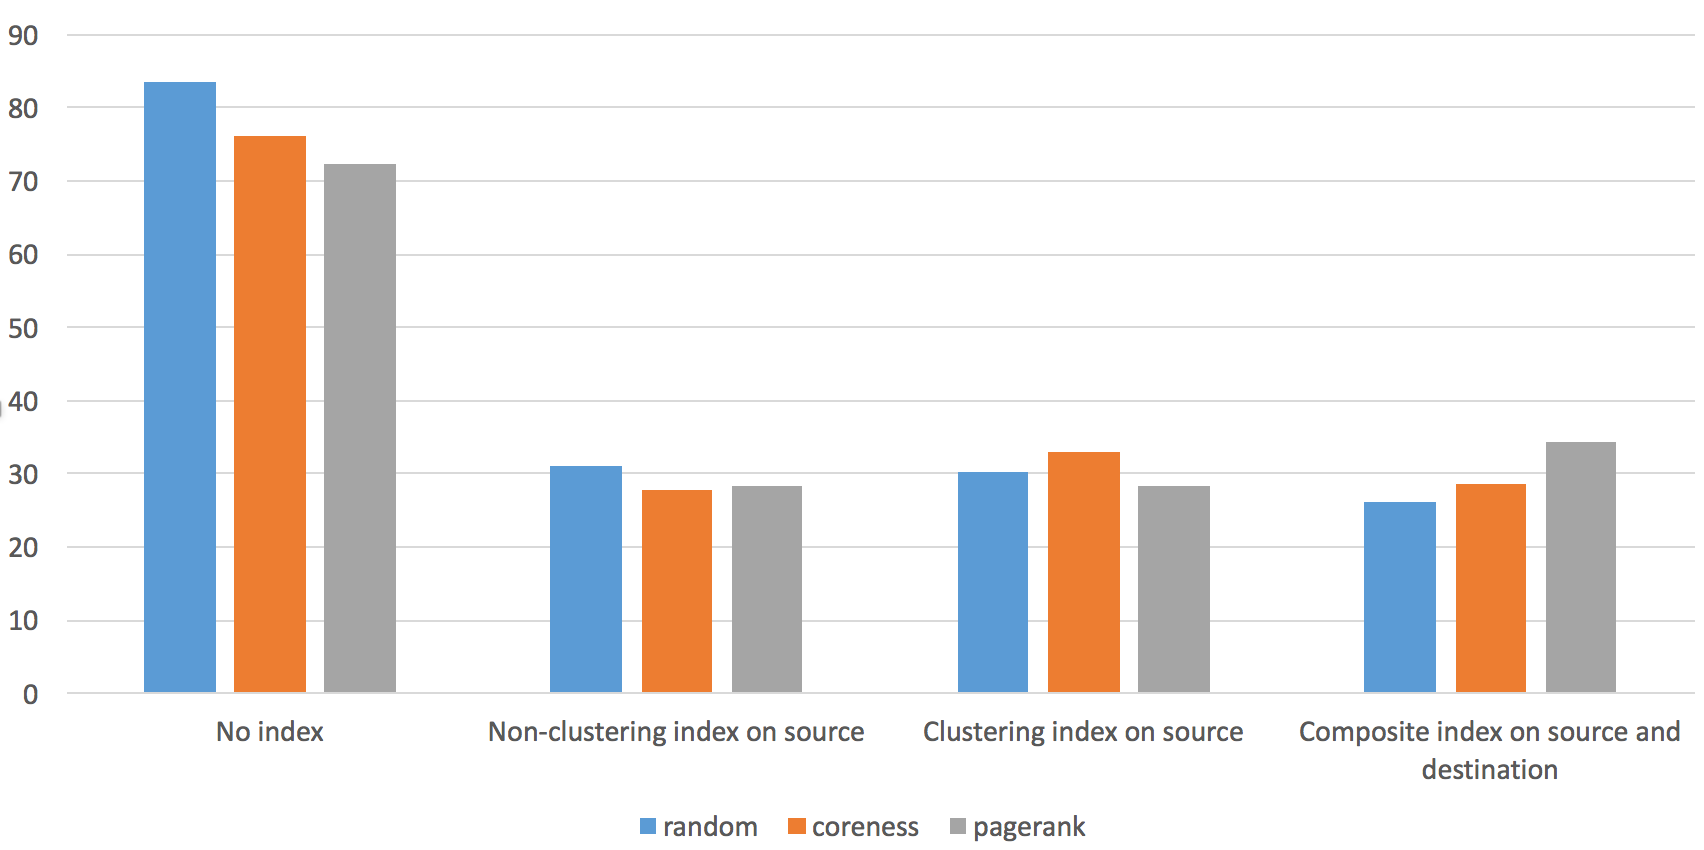
\includegraphics[width=0.8\linewidth]{fb}
\caption{Performance}
\end{figure}

\begin{figure}[H]
\centering
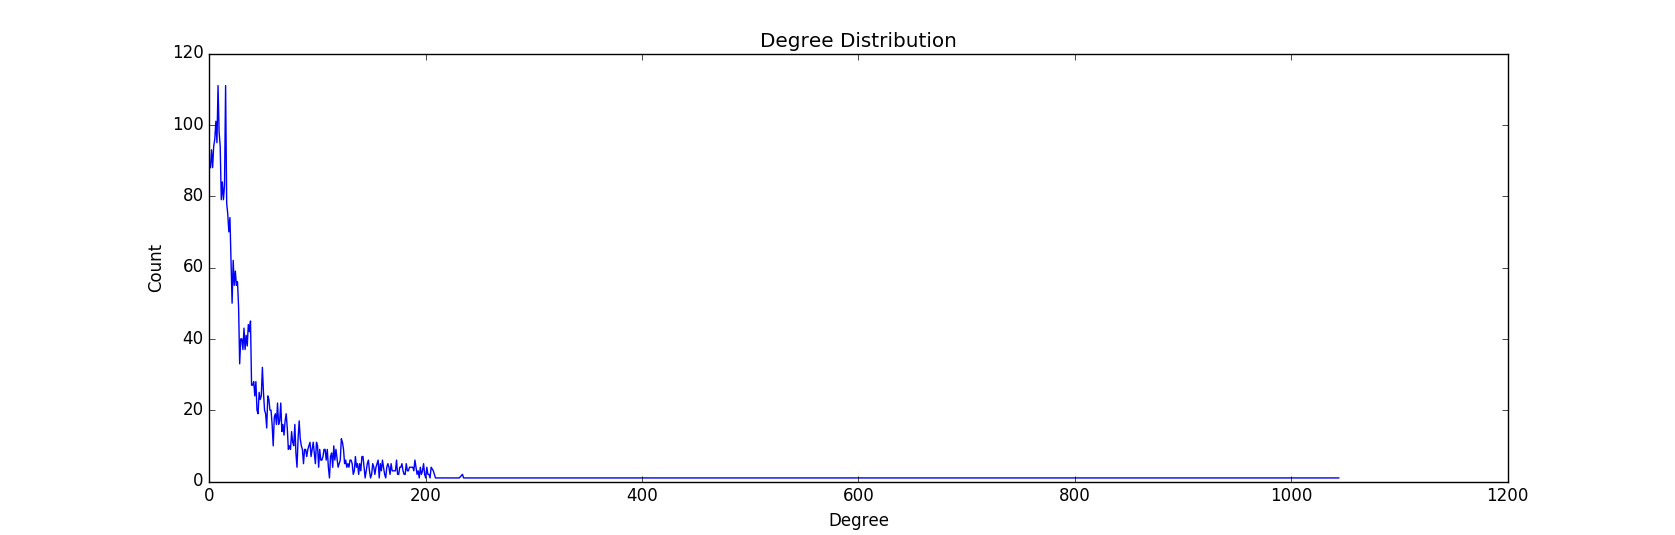
\includegraphics[width=1.0\linewidth]{fb_degree}
\caption{Degree Distribution}
\end{figure}

\begin{figure}[H]
\centering
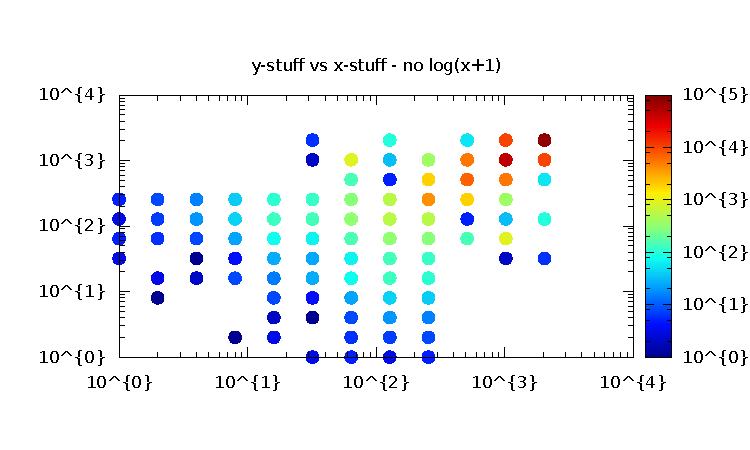
\includegraphics[width=0.8\linewidth]{core_scatter}
\caption{Scatter Plot}
\end{figure}

\subsubsection{Directed Social Network: Wiki Vote}

Wiki-Vote also belongs to social network dataset. From its degree distribution, we see it approximates power law and has relatively more edges. Majority of the nodes has small degrees while a few 'popular' has a degree over 1000. 

\begin{figure}[H]
\centering
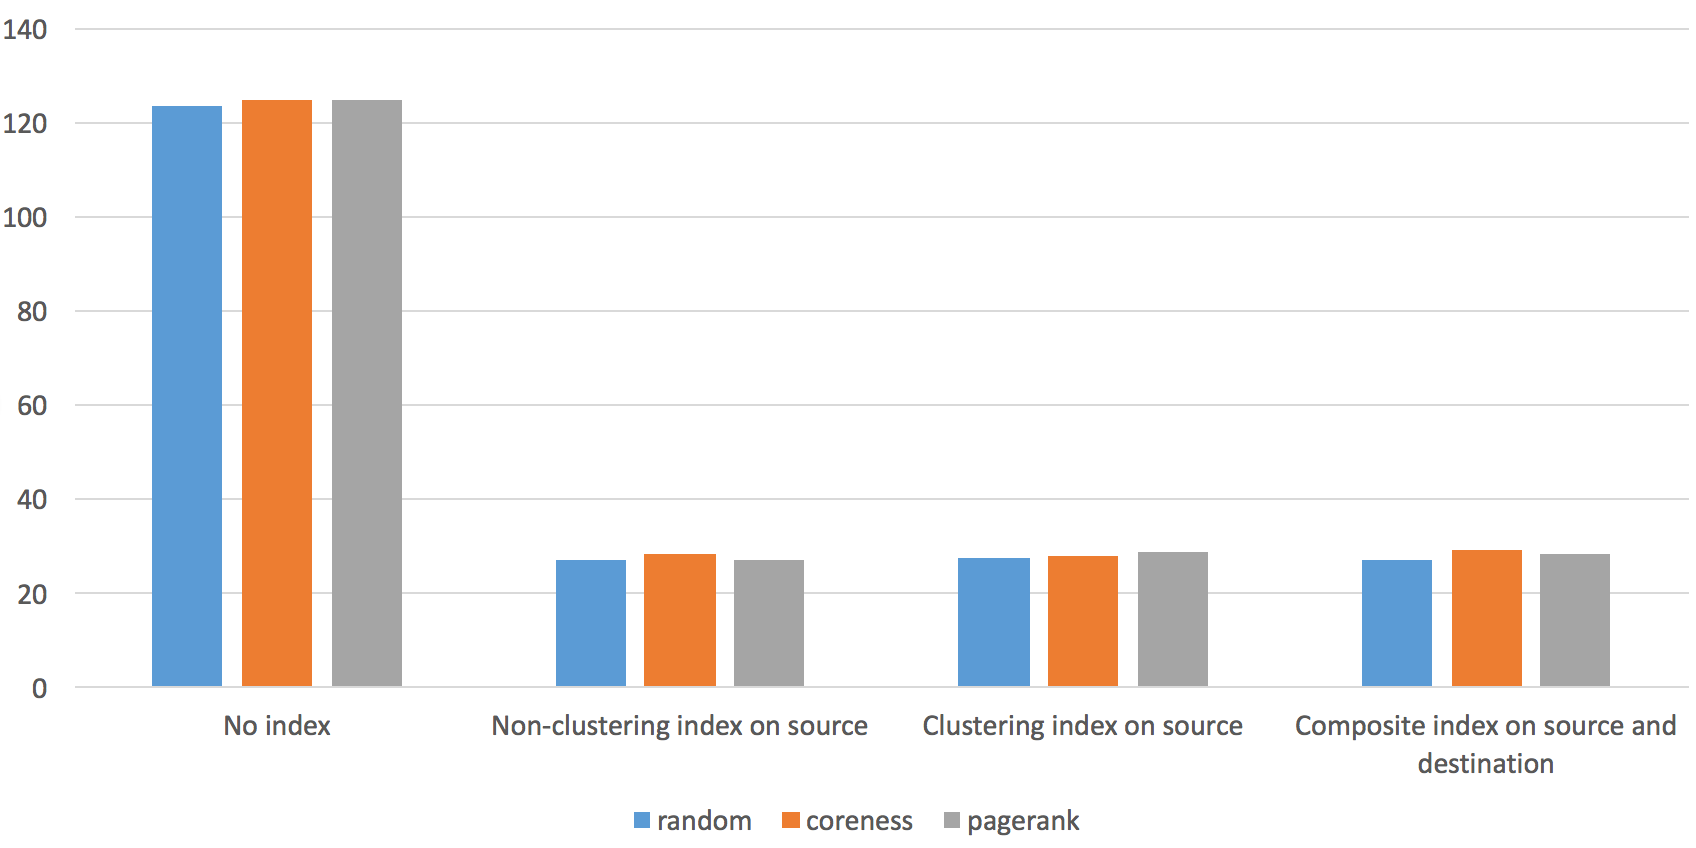
\includegraphics[width=0.8\linewidth]{wiki}
\caption{Performance}
\end{figure}

\begin{figure}[H]
\centering
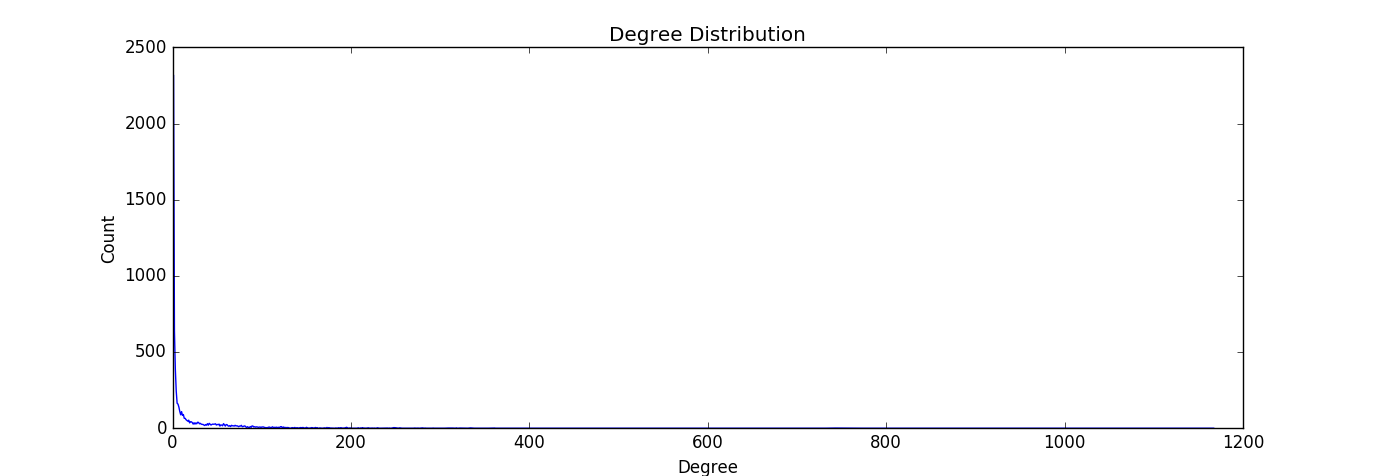
\includegraphics[width=1.0\linewidth]{wiki_degree}
\caption{Degree Distribution}
\end{figure}

\begin{figure}[H]
\centering
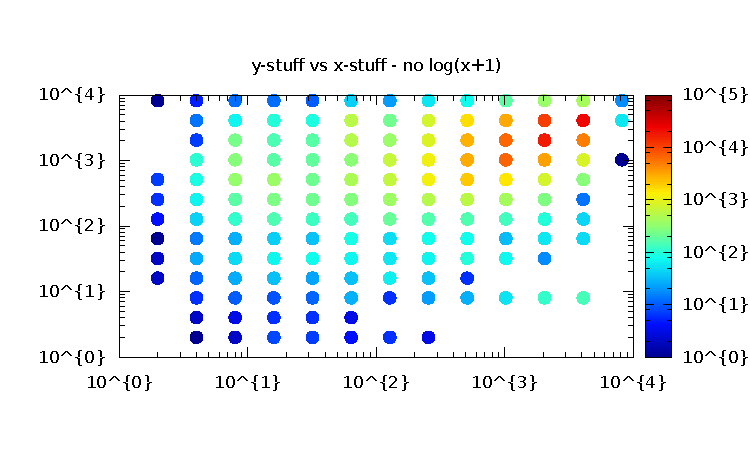
\includegraphics[width=0.8\linewidth]{wiki_scatter}
\caption{Scatter Plot}
\end{figure}

\subsubsection{Collaboration Network}
General Relativity and Quantum Cosmology collaboration network
\begin{figure}[H]
\centering
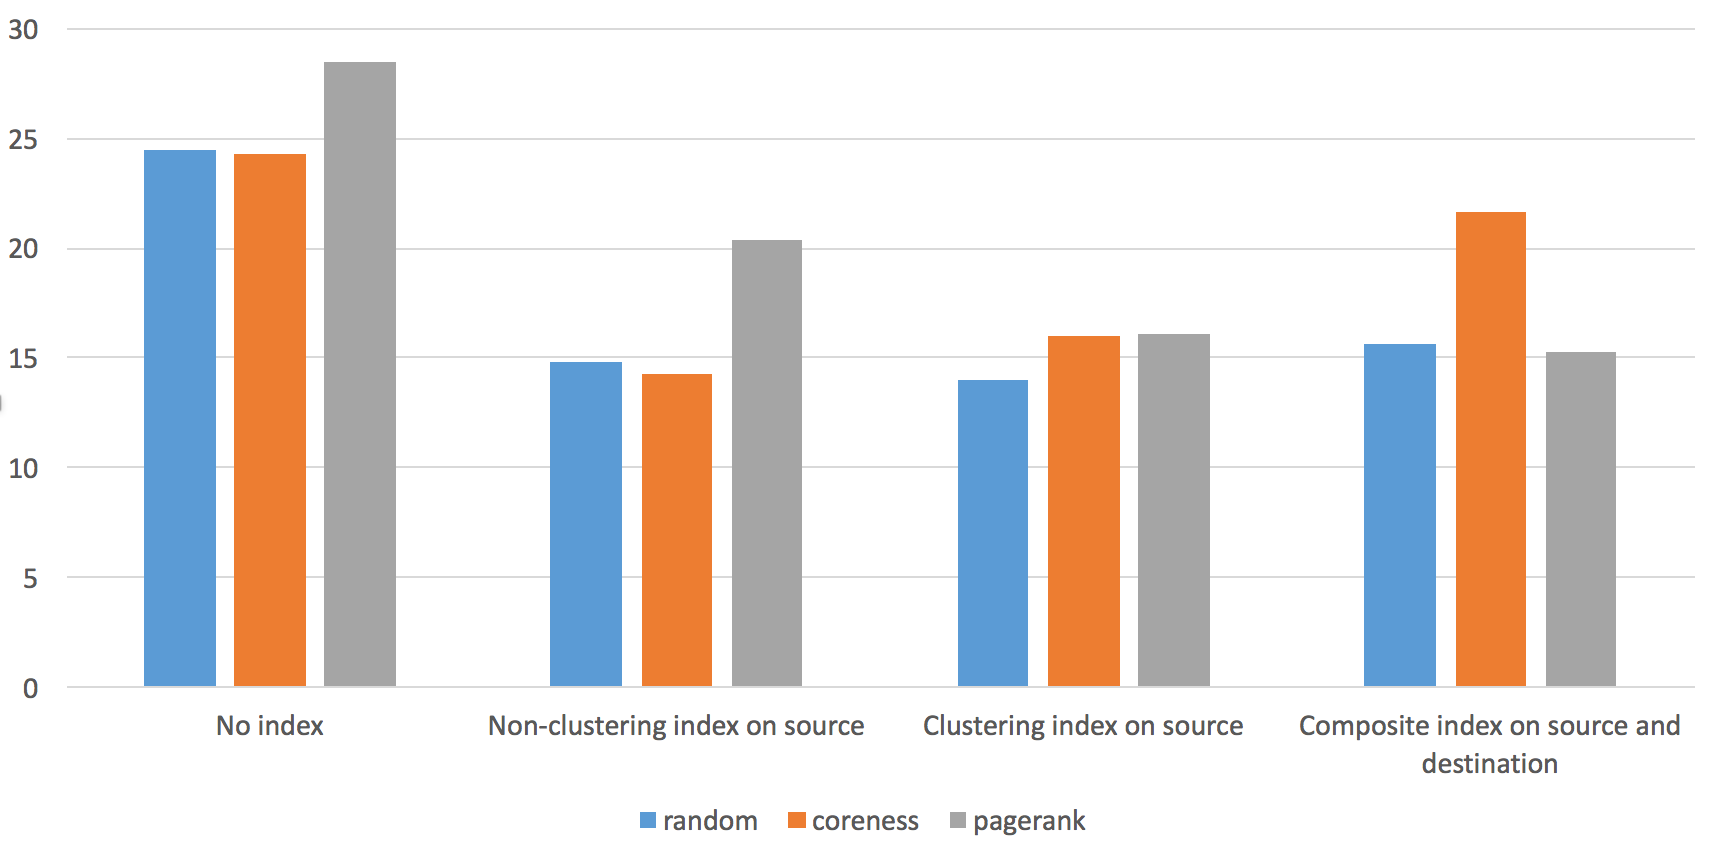
\includegraphics[width=0.8\linewidth]{co}
\caption{Performance}
\end{figure}
High Energy Physics - Theory collaboration network
\begin{figure}[H]
\centering
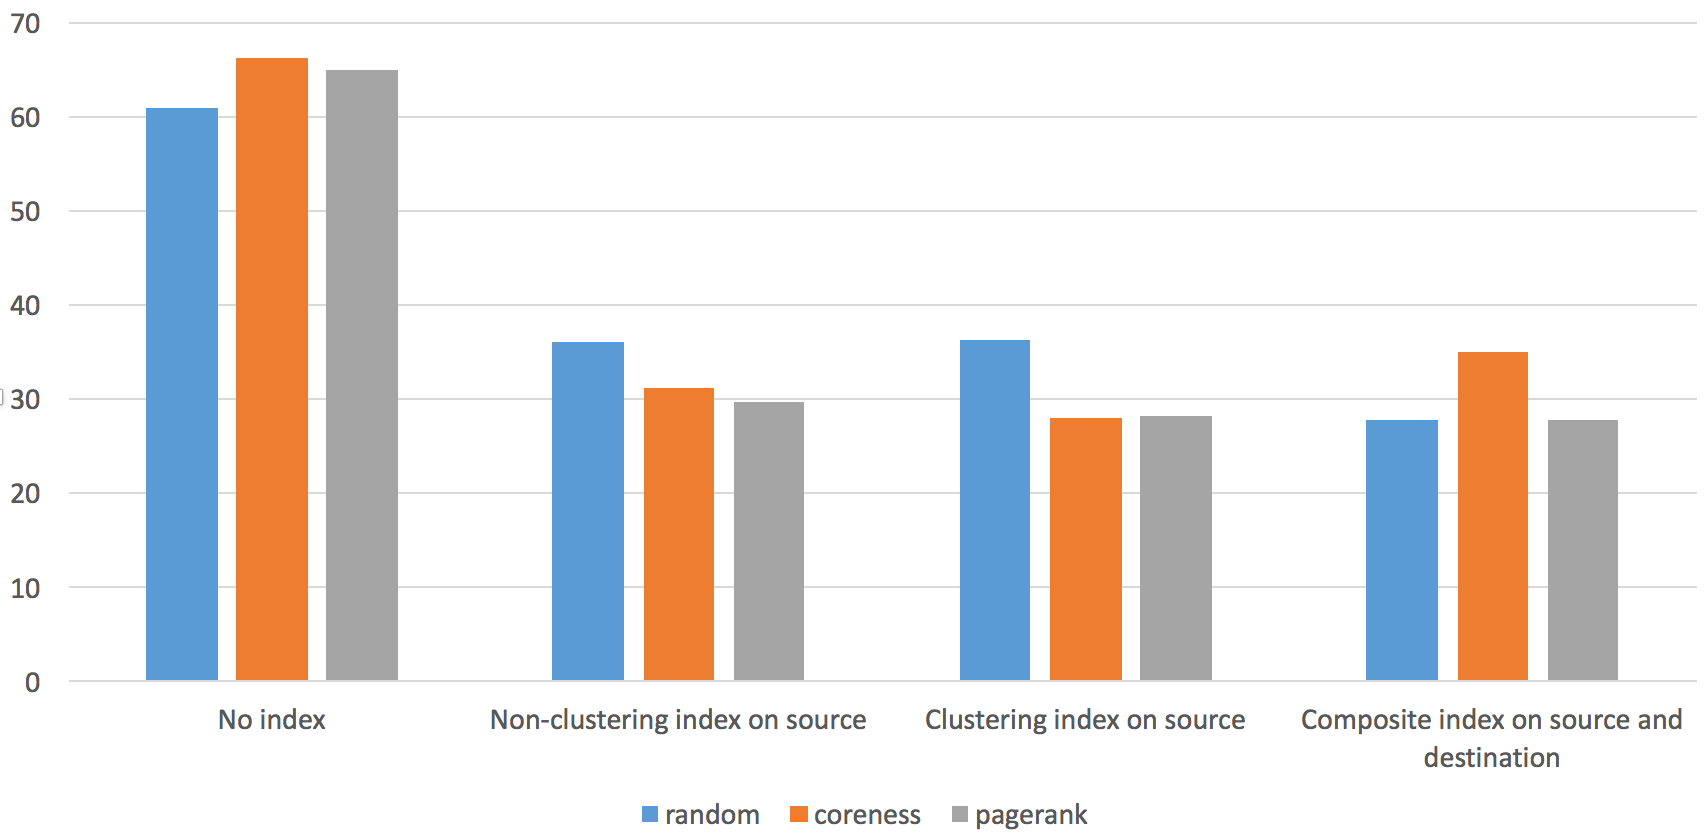
\includegraphics[width=0.8\linewidth]{ca}
\caption{Performance}
\end{figure}
Due to limited pages, we only list the degree distribution and scatter plot of General Relativity and Quantum Cosmology collaboration network as follows. They are quite similar.

\begin{figure}[H]
\centering
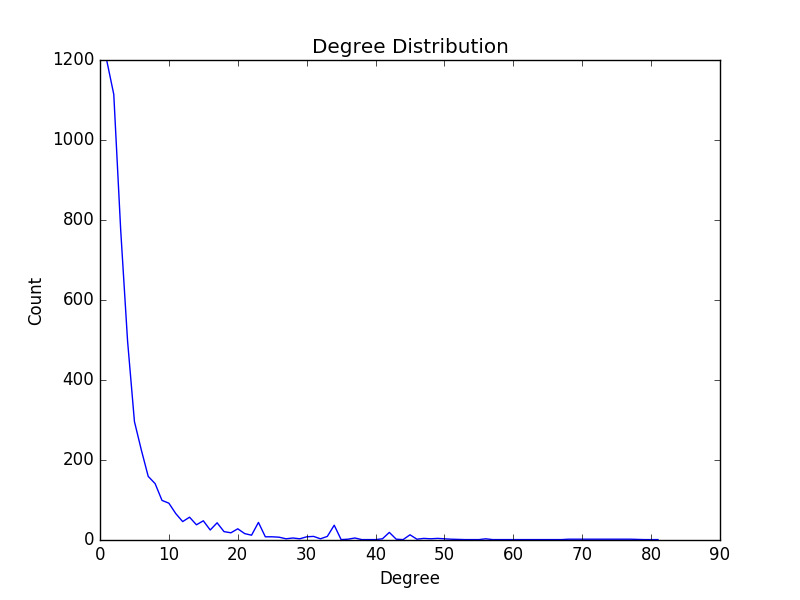
\includegraphics[width=0.6\linewidth]{ca_degree}
\caption{Degree Distribution}
\end{figure}

\begin{figure}[H]
\centering
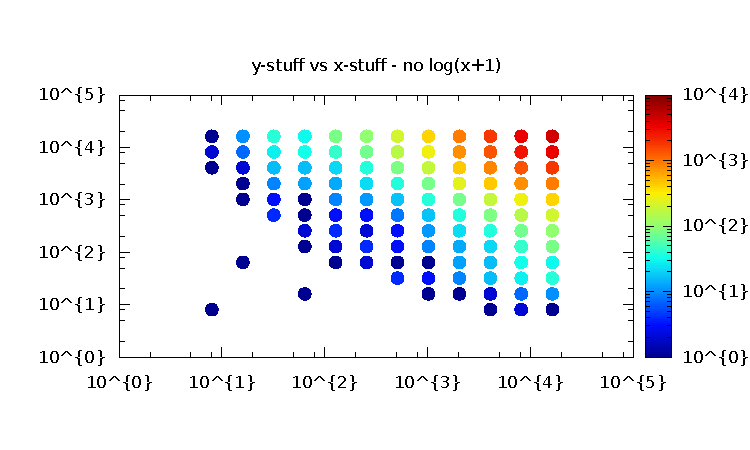
\includegraphics[width=0.8\linewidth]{ca_scatter}
\caption{Scatter Plot}
\end{figure}

\subsubsection{P2P Network}

\begin{figure}[H]
\centering
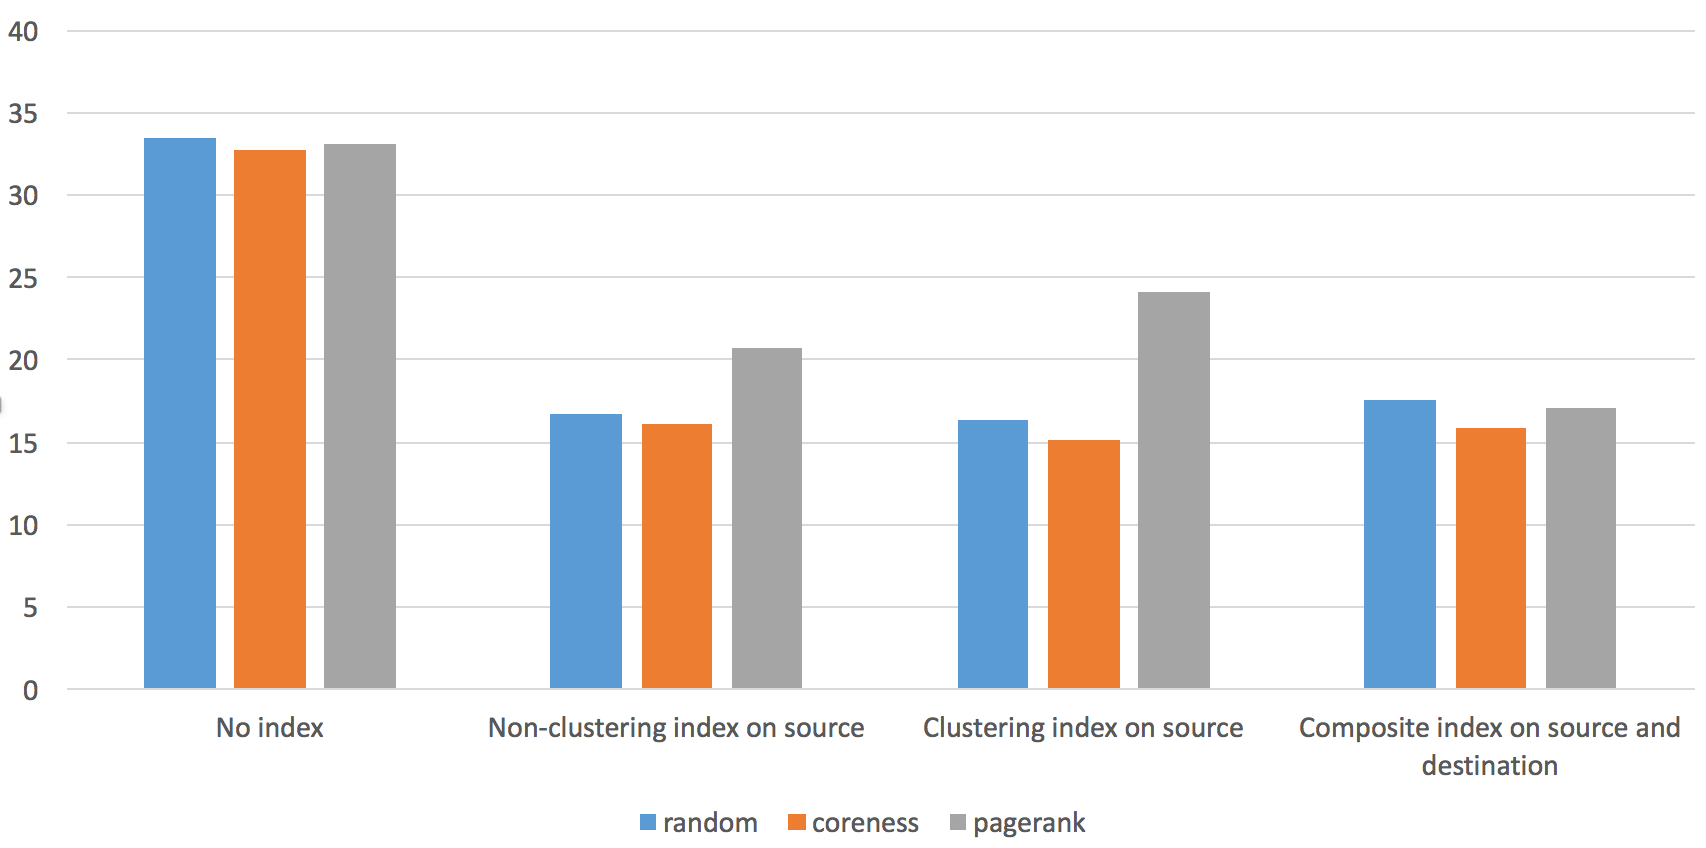
\includegraphics[width=0.8\linewidth]{p2p}
\caption{Performance}
\end{figure}

\begin{figure}[H]
\centering
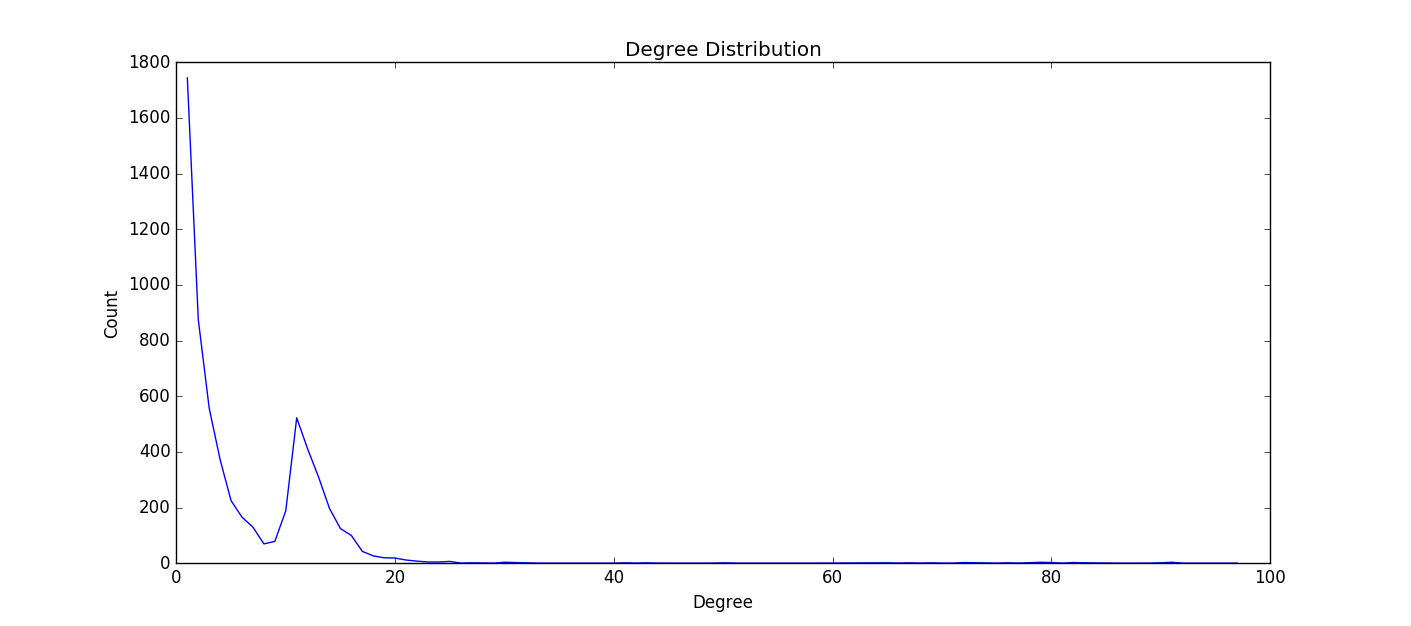
\includegraphics[width=0.8\linewidth]{p2p_degree}
\caption{Degree Distribution}
\end{figure}

\begin{figure}[H]
\centering
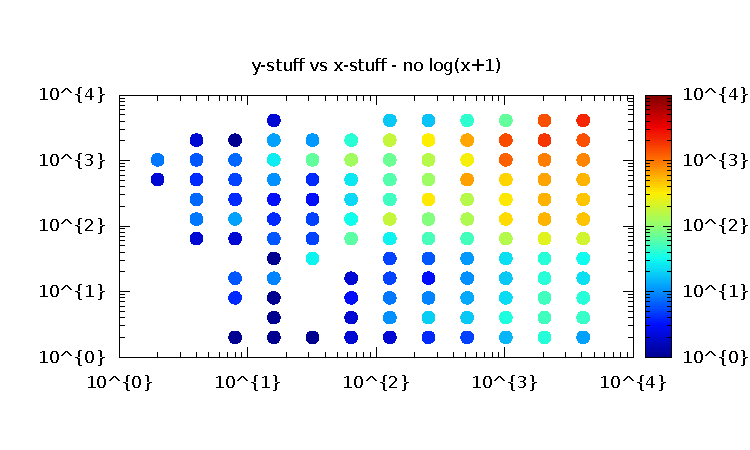
\includegraphics[width=0.8\linewidth]{p2p_scatter}
\caption{Scatter Plot}
\end{figure}

\subsection{Observation}

The most obvious result we can see from the experiment is that the running time get 2-4 times faster when using index. Degree of improvement depends on dataset types. \par

As for different types of index (clustering on source, non-clustering on source and composite index on source and destination), they all improve the running time and their impacts are similar. In some dataset e.g. Facebook, data with composite indexes run slightly faster. In other dataset like wiki-Vote ranked by coreness, clustering index gives a slightly better performance. So the performance of different indexes is dependent on dataset. \par

Clustering index stores actual rows on the disc and search for actual rows while non-clustered index store pointers and pointers point to where actual rows are stored. Generally clustering index would provide a faster way of searching, but in our experiment, we not only have searching, but also a huge amount of work of deleting, which may slow down using clustering index. \cite{MSR} \par

We also experiment on preprocessing the data, ranking the source node id in the initial dataset by coreness and page rank. And we find out there is not much difference in running time when we reorder the dataset first. Adding indexes to the reordered dataset also show similar trend as the original random data. \par

Another interesting finding is that the five datasets we use have different number of nodes and edges, but the running time of the algorithm is not proportional to the number of nodes. For example, ca-HepTh dataset has 9877 nodes while Facebook has 4024 nodes; however, the raw running time of Facebook is 83s while ca-HepTh is 61s. But when we look at their edges, we find that the edges in Facebook is 88234, almost 4 times the edges in ca-HepTh. So we may say that the number of edges determines the running time. In addition, as we look at dataset wiki-Vote, it has the largest number of edges: 103,689, and we see the raw running time is longer than the other datasets. Surprisingly, after adding index to it, the running time decreases dramatically from 123s to 27s, even shorter than the other datasets. \par
